\documentclass[tikz]{standalone}
\usepackage{fontspec}
\renewcommand*{\familydefault}{\sfdefault}
\usepackage{standalone}
\usepackage{amssymb}
\usetikzlibrary{decorations}
\usetikzlibrary{arrows.meta, decorations.pathmorphing, decorations.pathreplacing, shapes.geometric}
\usetikzlibrary{bayesnet}

\begin{document}

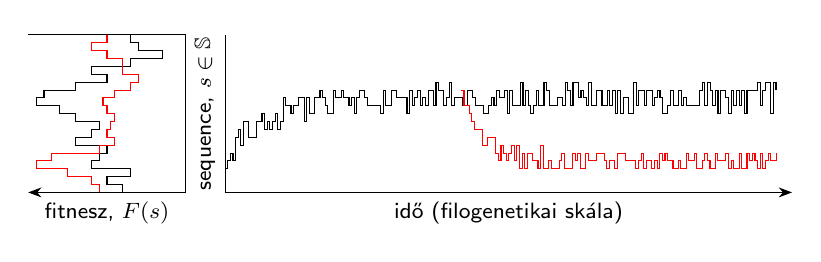
\begin{tikzpicture}[font=\footnotesize]

\draw[-Stealth] (0,-1) -- node[anchor=north] {idő (filogenetikai skála)} (7.2,-1) ;
\draw[xshift=-0.0 cm] (0,-1) -- node[rotate=90, anchor=south]
{sequence, \(s\in\mathbb{S}\)} (0,1) ;
\draw[-Stealth, xshift=-0.5 cm] (0,-1) -- node[anchor=north] {fitnesz, \(F(s)\)} (-2,-1) ;
\draw[xshift=-0.5 cm] (0,1) -- (-2,1) ;
\draw[xshift=-0.5 cm] (0,-1) -- (0,1) ;

% fitness landscape
\draw[rotate=90, yshift=0.5 cm] plot[const plot] coordinates {
(-1.0,0.8) (-0.9,1.0) (-0.8,0.7) (-0.7,1.2) (-0.6,1.1) (-0.5,1.0) (-0.4,1.4) (-0.3,1.2) (-0.2,1.1) (-0.1,1.4) (0.0,1.6) (0.1,1.9) (0.2,1.8) (0.3,1.4) (0.4,1.0) (0.5,1.2) (0.6,0.7) (0.7,0.3) (0.8,0.6) (0.9,0.7) (1.0,0.7)
};

% evol. trajectory
\draw[domain=0:7, samples=210]
%plot (\x, {- 0.8 * exp(-2 * \x) + 0.1 * rand + 0.2 }) 
plot[const plot] (\x, {round((- 0.8 * exp(-2 * \x) + 0.2 * rand + 0.2) * 10) / 10 })
;
\path
(3.5,0.2) coordinate (zoomleft)
(3.6,0.2) coordinate (zoomright)
;

% ADAPTATION
\begin{scope}[red]
% evol. trajectory
\draw[domain=3:7, samples=120]
plot[const plot] (\x, {round(( 0.9 * exp(-4 * (\x - 3)) + 0.15 * rand - 0.6) * 10) / 10 })
;

% fitness landscape
\draw[rotate=90, yshift=0.5 cm] plot[const plot] coordinates {
(-1.0,1.1) (-0.9,1.2) (-0.8,1.5) (-0.7,1.9) (-0.6,1.7) (-0.5,1.1) (-0.4,0.9)
(-0.3,1.0) (-0.2,0.95) (-0.1,0.9) (0.0,1.0) (0.1,1.05) (0.2,0.9) (0.3,0.7) (0.4,0.6) (0.5,0.8) (0.6,0.8) (0.7,1.0) (0.8,1.2) (0.9,1.0) (1.0,1.0)
};

\end{scope}

\end{tikzpicture}

\end{document}
% POPULATION GENETICS
\begin{scope}[yshift=3 cm]
\draw[-Stealth] (0,-1) coordinate (popleft) -- node[anchor=north]
{time (population genetic~scale)} (7.2,-1) coordinate (popright) ;
\draw[xshift=-0.0 cm] (0,-1) -- node[rotate=90, anchor=south]
{szekvencia, \(s\in\mathbb{S}\)} (0,1) ;
\draw[dotted]
(zoomleft) ..controls +(90:1.0) and +(-15:3) .. (popleft)
(zoomright) ..controls +(90:1.0) and +(-165:3) .. (popright)
%(zoomleft) to[out=90, in=-30] (popleft)
;

\draw[blue, xshift=-1.5 cm, pin distance=0.1 cm, inner sep=0, minimum size=0] (0,-1.0) node[pin={right:0}] {} -- node[rotate=90, anchor=south,
align=center]
{mutant allele\\frequency}(0,1.0) node[pin={right:\(2N\)}] {};
\draw[blue, xshift=-1.0 cm]
;

% substitutions
\path[inner sep=0]
(0,0.7) node (s0) {}
(1,0.3) node (s1) {}
(5,0.5) node (s2) {}
(7,0.5) node (s3) {}
;

\draw plot[const plot] coordinates {
(s0) (s1) (s2) (s3)
}
;

\draw[blue, samples=25, xscale=0.05, domain=10:20] plot (\x, {2 * exp(\x - 15) / (1 + exp(\x - 15) + 0.5 * rand) - 1});
\draw[blue, samples=50, xscale=0.10, domain=30:50]
plot (\x, {2 * exp(\x - 45) / (1 + exp(\x - 45) + 0.5 * rand) - 1});
\draw[blue, samples=25, xscale=0.10, domain=20:25]
plot (\x, { sin((\x - 20) * pi * 11.0) +  0.1 * rand) - 1});

% event labels
\begin{scope}[gray]
\path
(3,1) node[anchor=north] (subst) {substitutions}
(3,1) node[anchor=south] (fix) {mutant fixations}
(2.5,-0.0) node[anchor=west] (refix) {re-fixation}
;
\end{scope}

% label arrows
\begin{scope}[-Stealth, gray, very thin]
\draw (refix) to[] (2.5,-1);
\draw (subst.west) to[bend right] (s1);
\draw (subst.east) to[bend left] (s2);
\draw (fix.west) to[bend right] (1,1);
\draw (fix.east) to[bend left] (5,1);
\end{scope}
\end{scope}

% ADAPTATION
\begin{scope}[red]
% evol. trajectory
\draw[domain=3:7, samples=120]
plot[const plot] (\x, {round(( 0.9 * exp(-4 * (\x - 3)) + 0.2 * rand - 0.7) * 10) / 10 })
;

% fitness landscape
\draw[rotate=90, yshift=0.5 cm] plot[const plot] coordinates {
(-1.0,0.6) (-0.9,0.5) (-0.8,0.3) (-0.7,0.3) (-0.6,0.9) (-0.5,0.8) (-0.4,0.9) (-0.3,1.0) (-0.2,1.0) (-0.1,0.9) (0.0,1.3) (0.1,1.7) (0.2,2.1) (0.3,1.9) (0.4,1.1) (0.5,1.7) (0.6,1.3) (0.7,1.4) (0.8,1.2) (0.9,1.0) (1.0,1.0)
};

